\section{Results}
\subsection{Stock analysis}
\begin{figure}[H]
    \centering
    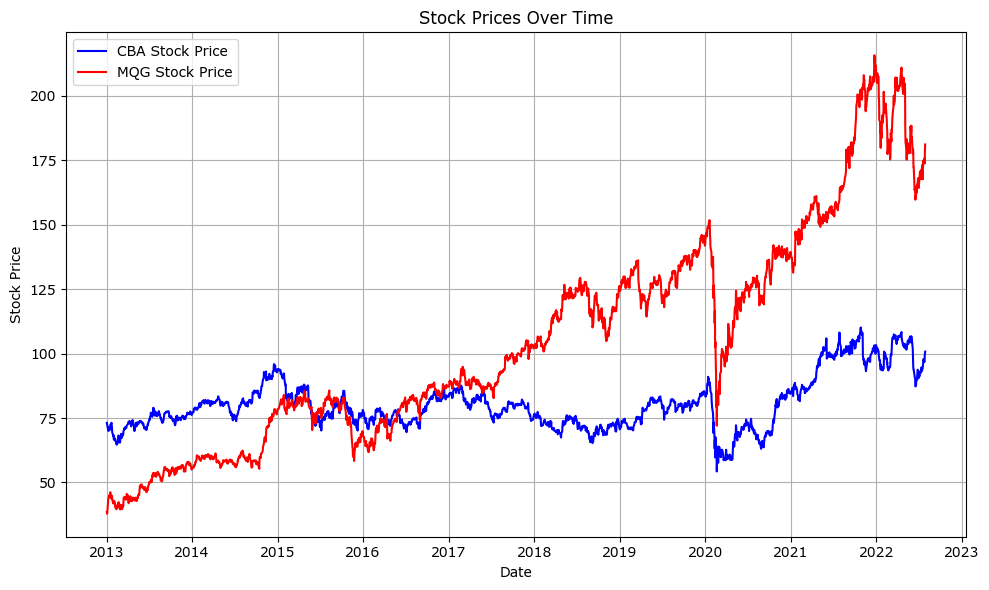
\includegraphics[width=1\linewidth]{image/time_series.png}
    \caption{Time series of stock}
    \label{fig:Time_series_stock}
\end{figure}
From the time series of the stock price, we can see that these two stocks do exhibit some positive correlation.
\begin{itemize}
    \item The MQG stock has a significant increasing trend over time, However, it decreased during 2020, which may due to the effects of COVID-19. But at the end, it has been recovered since then and fluctuated in these recent years. Due to large movement of the stock price in the near future but insecure of the direction, this strategy will efficient for the MQG stock with the required maturity.
    \item The CBA stock does not have a clear increasing trend over the time. Only after the COVID recovery where the stock went up higher than it used to be in previous years, this stock seems to fluctuate around. However, when taking it closer to the time series, we can see that the stock price of CBA seems to increase when it is closer to the end of the year and decrease at the beginning of the year. With the butterfly spread, if helps earning payoff with small upward movement of the stock. This one is perfectly fit with what is exhibiting in the CBA stock where it's reaching to the end of the year and most of the movement of the CBA stock seeming not to be to large.
\end{itemize}
\subsection{Dependence structure}
\begin{figure}[H]
    \centering
    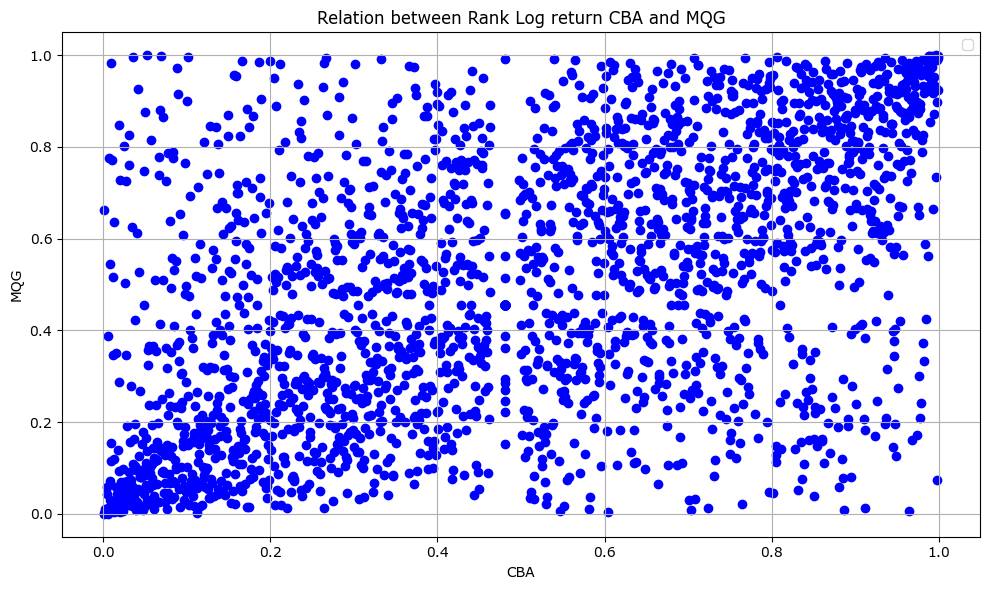
\includegraphics[width=1\linewidth]{image/dependence_structure.png}
    \caption{Rank Dependence structure}
    \label{fig:Rank Dependence structure}
\end{figure}
From the plot above, we can see that these two stock are heavily tail dependence. Furthermore, when performing statistical correlation, it does show that these two stock shows significantly high correlation. This helps with consolidation the probability to receive profit in the future as both stocks seems to having an increasing trend.
\begin{table}[H]
    \centering
    \begin{tabular}{@{} l c @{}}
        \toprule
        \textbf{Metric} & \textbf{Value} \\
        \midrule
        Pearson Linear Correlation & 0.5747 \\
        Spearman Correlation & 0.5342 \\
        Kendall's tau & 0.3883 \\
        Spearman Rank Correlation & 0.5342 \\
        Lower Tail Dependence (5\%) & 0.4146 \\
        Upper Tail Dependence (95\%) & 0.3416 \\
        \bottomrule
    \end{tabular}
    \caption{Correlation and Dependence Statistics}
    \label{tab:correlation_dependence}
\end{table}
\subsection{Portfolio valuation}
\begin{table}[H]
    \centering
    \begin{tabular}{@{} l c @{}}
        \toprule
        \textbf{Portfolio} & \textbf{Total Value} \\
        \midrule
        CBA Portfolio & 11.1068 \\
        MQG Portfolio & 5.1034 \\
        \midrule
        \textbf{Total Portfolio Value} & \textbf{16.2102} \\
        \bottomrule
    \end{tabular}
    \caption{Portfolio Values}
    \label{tab:portfolio_values}
\end{table}
\subsection{Portfolio risk measure}
\subsubsection{Diversified portfolio}
\begin{table}[H]
    \centering
    \begin{tabular}{@{} l c c c @{}}
        \toprule
        \textbf{Risk measure} & \textbf{90.0\%} & \textbf{95.0\%} & \textbf{99.0\%} \\
        \midrule
        1 day VaR & 0.410077 & 0.529050 & 0.752223 \\
        10 day VaR Scale & 1.231125 & 1.607351 & 2.313088 \\
        10 day VaR Overlapping & 1.238867 & 1.615405 & 2.321728 \\
        10 day VaR Non-Overlapping & 1.256377 & 1.640089 & 2.359867 \\
        1 day ES & 0.565115 & 0.665889 & 0.863194 \\
        10 day ES Scale & 1.721398 & 2.040074 & 2.664008 \\
        10 day ES Overlapping & 1.729547 & 2.048488 & 2.672940 \\
        10 day ES Non-Overlapping & 1.756405 & 2.081422 & 2.717770 \\
        \bottomrule
    \end{tabular}
    \caption{Method 1: Risk measurement for diversified portfolio}
    \label{tab:method_1_diversified_port}
\end{table}
\begin{table}[H]
    \centering
    \begin{tabular}{@{} l c c c | c c c @{}}
        \toprule
        &\multicolumn{3}{c}{Method 2}&\multicolumn{3}{c}{Method 3}\\
        \textbf{Risk measure} & \textbf{90.0\%} & \textbf{95.0\%} & \textbf{99.0\%}& \textbf{90.0\%} & \textbf{95.0\%} & \textbf{99.0\%} \\
        \midrule
        1 day VaR & 0.275572 & 0.386402 & 0.621234 & 0.235908 & 0.412731 & 0.617628\\
        10 day VaR & 0.658272 & 0.973303 & 2.373378 & 0.695137 & 2.523439 & 3.161269 \\
        1 day ES & 0.445255 & 0.566174 & 0.902753 & 0.432510 & 0.579034 & 0.730826 \\
        10 day ES & 1.236436 & 1.678773 & 3.073507 & 2.210965 & 2.968621 & 3.358309 \\
        \bottomrule
    \end{tabular}
    \caption{Method 2 and 3: Risk measurement for diversified portfolio}
    \label{tab:method_2_and_3_diversified_port}
\end{table}
\begin{table}[H]
    \centering
    \begin{tabular}{@{} l c c c | c c c @{}}
        \toprule
        &\multicolumn{3}{c}{Method 4}&\multicolumn{3}{c}{Method 5}\\
        \textbf{Risk measure} & \textbf{90.0\%} & \textbf{95.0\%} & \textbf{99.0\%}& \textbf{90.0\%} & \textbf{95.0\%} & \textbf{99.0\%} \\
        \midrule
        1 day VaR & 0.342544 & 0.435994 & 0.615092 & 0.392433 & 0.544621 & 0.993045 \\
        10 day VaR Scale & 0.821668 & 1.179754 & 1.937240 & 0.909562 & 1.491127 & 3.645028 \\
        10 day VaR Overlapping & 0.784553 & 1.116975 & 1.826953 & 0.392433 & 0.544621 & 0.993045 \\
        10 day VaR Non-Overlapping & 0.805565 & 1.145943 & 1.862641 & 0.839188 & 1.299698 & 2.623053 \\
        1 day ES & 0.465564 & 0.545898 & 0.705629 & 0.673422 & 0.888084 & 1.647978 \\
        10 day ES Scale & 1.311487 & 1.642349 & 2.358310 & 2.260437 & 3.361677 & 8.107745 \\
        10 day ES Overlapping & 1.242389 & 1.552546 & 2.216193 & 0.673422 & 0.888084 & 1.647978 \\
        10 day ES Non-Overlapping & 1.270938 & 1.585463 & 2.259616 & 1.616946 & 2.192836 & 3.949307 \\
        \bottomrule
    \end{tabular}
    \caption{Method 4 and 5: Risk measurement for diversified portfolio}
    \label{tab:method_4_and_5_diversified_port}
\end{table}
\subsubsection{Undiversified portfolio}
\begin{table}[H]
    \centering
    \begin{tabular}{@{} l c c c | c c c @{}}
        \toprule
        &\multicolumn{3}{c}{CBA portfolio}&\multicolumn{3}{c}{MQG portfolio}\\
        \textbf{Risk measure} & \textbf{90.0\%} & \textbf{95.0\%} & \textbf{99.0\%}& \textbf{90.0\%} & \textbf{95.0\%} & \textbf{99.0\%} \\
        \midrule
        1 day VaR                & 0.210565 & 0.270722 & 0.383568 & 0.252151 & 0.325889 & 0.464210\\
        10 day VaR Scale         & 0.654649 & 0.844883 & 1.201731 & 0.742936 & 0.976117 & 1.413524\\
        10 day VaR Overlapping    & 0.635220 & 0.819840 & 1.166157 & 0.761058 & 0.997600 & 1.441314\\
        10 day VaR Non-Overlapping & 0.647901 & 0.836415 & 1.190035 & 0.757741 & 0.995253 & 1.440786\\
        1 day ES                 & 0.288958 & 0.339914 & 0.439679 & 0.348242 & 0.410701 & 0.532988\\
        10 day ES Scale          & 0.902550 & 1.063685 & 1.379170 & 1.046802 & 1.244314 & 1.631021\\
        10 day ES Overlapping      & 0.875805 & 1.032185 & 1.338359 & 1.069304 & 1.269664 & 1.661946\\
        10 day ES Non-Overlapping  & 0.893560 & 1.053238 & 1.365870 & 1.067252 & 1.268432 & 1.662323\\ \bottomrule
    \end{tabular}
    \caption{Method 1: Risk measurement for undiversified portfolio}
    \label{tab:method_1_undiversified_port}
\end{table}
\begin{table}[H]
    \centering
    \begin{tabular}{@{} l c c c | c c c @{}}
        \toprule
        &\multicolumn{3}{c}{CBA portfolio}&\multicolumn{3}{c}{MQG portfolio}\\
        \textbf{Risk measure} & \textbf{90.0\%} & \textbf{95.0\%} & \textbf{99.0\%}& \textbf{90.0\%} & \textbf{95.0\%} & \textbf{99.0\%} \\
        \midrule
        1 day VaR                & 0.187872 & 0.292862 & 0.581258 & 0.130495 & 0.153262 & 0.163198\\
        10 day VaR         & 0.756976 & 1.128512 & 3.374953 & 0.149145 & 0.160246 & 0.163769\\
        1 day ES                & 0.378911 & 0.523161 & 1.068029 & 0.150610 & 0.160025 & 0.163622\\
        10 day ES          & 1.766399 & 2.627849 & 6.208862 & 0.158665 & 0.162676 & 0.163871\\\bottomrule
    \end{tabular}
    \caption{Method 2: Risk measurement for undiversified portfolio}
    \label{tab:method_2_undiversified_port}
\end{table}
\begin{table}[H]
    \centering
    \begin{tabular}{@{} l c c c | c c c @{}}
        \toprule
        &\multicolumn{3}{c}{CBA portfolio}&\multicolumn{3}{c}{MQG portfolio}\\
        \textbf{Risk measure} & \textbf{90.0\%} & \textbf{95.0\%} & \textbf{99.0\%}& \textbf{90.0\%} & \textbf{95.0\%} & \textbf{99.0\%} \\
        \midrule
        1 day VaR                & 0.239767 & 0.319632 & 0.481923 & 0.149994 & 0.160156 & 0.163752\\
        10 day VaR Scale         & 0.938897 & 1.321099 & 2.166147 & 0.149072 & 0.160170 & 0.163778\\
        10 day VaR Overlapping    & 0.902745 & 1.267549 & 2.072635 & 0.148908 & 0.160120 & 0.163757\\
        10 day VaR Non-Overlapping & 0.926351 & 1.306488 & 2.129014 & 0.148760 & 0.160086 & 0.163762\\
        1 day ES                 & 0.348173 & 0.420330 & 0.571202 & 0.159045 & 0.162638 & 0.163865\\
        10 day ES Scale          & 1.479058 & 1.847924 & 2.670337 & 0.158945 & 0.162705 & 0.163873\\
        10 day ES Overlapping      & 1.418766 & 1.770616 & 2.553771 & 0.158895 & 0.162628 & 0.163865\\
        10 day ES Non-Overlapping  & 1.458601 & 1.822423 & 2.633733 & 0.158810 & 0.162620 & 0.163870\\ \bottomrule
    \end{tabular}
    \caption{Method 4: Risk measurement for undiversified portfolio}
    \label{tab:method_4_undiversified_port}
\end{table}
\subsection{Portfolio risk measure at 95\% confidence}
\begin{table}[H]
    \centering
    \begin{tabular}{@{} c l c c c c c c@{}}
        \toprule
        \textbf{M} &\textbf{Risk measure} & {\textbf{CBA port.}} & \textbf{MQG port.} & \textbf{Sum of risk} & \textbf{Total port.}\\
        \midrule
        \multirow{8}{*}{1}&1 day VaR & 0.270722 & 0.325889 & 0.596611 & 0.529050 \\
        &10 day VaR Scale & 0.844883 & 0.976117 & 1.821000 & 1.607351 \\
        &10 day VaR Overlapping & 0.819840 & 0.997600 & 1.817440 & 1.615405 \\
        &10 day VaR Non-Overlapping & 0.836415 & 0.995253 & 1.831668 & 1.640089 \\
        &1 day ES & 0.339914 & 0.410701 & 0.750615 & 0.665889 \\
        &10 day ES Scale & 1.063685 & 1.244314 & 2.307999 & 2.040074 \\
        &10 day ES Overlapping & 1.032185 & 1.269664 & 2.301849 & 2.048488 \\
        &10 day ES Non-Overlapping & 1.053238 & 1.268432 & 2.321670 & 2.081422 \\
        \midrule
        \multirow{4}{*}{2}&1 day VaR & 0.292862 & 0.153262 & 0.446124 & 0.386402 \\
        &10 day VaR & 1.128512 & 0.160246 & 1.288758 & 0.973303 \\
        &1 day ES & 0.523161 & 0.160025 & 0.683186 & 0.566174 \\
        &10 day ES & 2.627849 & 0.162676 & 2.790525 & 1.678773 \\
        \midrule
        \multirow{8}{*}{4}&1 day VaR & 0.319632 & 0.160156 & 0.479788 & 0.435994 \\
        &10 day VaR Scale & 1.321099 & 0.160170 & 1.481269 & 1.179754 \\
        &10 day VaR Overlapping & 1.267549 & 0.160120 & 1.427669 & 1.116975 \\
        &10 day VaR Non-Overlapping & 1.306488 & 0.160086 & 1.466574 & 1.145943 \\
        &1 day ES & 0.420330 & 0.162638 & 0.582968 & 0.545898 \\
        &10 day ES Scale & 1.847924 & 0.162705 & 2.010629 & 1.642349 \\
        &10 day ES Overlapping & 1.770616 & 0.162628 & 1.933244 & 1.552546 \\
        &10 day ES Non-Overlapping & 1.822423 & 0.162620 & 1.985043 & 1.585463 \\
        \bottomrule
    \end{tabular}
    \caption{Risk measure comparison}
    \label{tab:risk_measure_comparison}
\end{table}